\section{Generování signálu}

Byl vygenerován zvukový soubor obsahující pouze rušení složený z cosinusovek frekvencí, které jsme našli pomocí funkcí z knihovny numpy. Tento signál byl poté podroben spektrální analýze.
Z výskedků této analýzy můžeme viděť, že náš odhad byl správný a frekvence +- odpovídají.

\begin{figure}[H] 
	\centering
	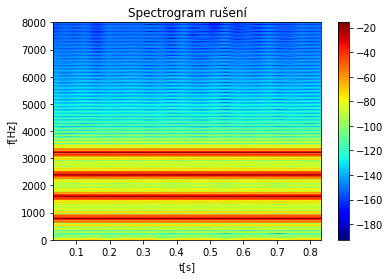
\includegraphics[scale=0.67,keepaspectratio]{Figure_8}
	\caption{Výkonový spektrogram rušení}
\end{figure}

\begin{figure}[H] 
	\centering
	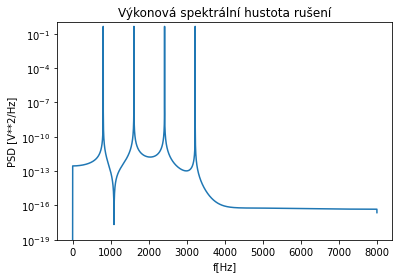
\includegraphics[scale=0.67,keepaspectratio]{Figure_9}
	\caption{Výkonová spektrální hustota rušení}
\end{figure}

\begin{landscape}
\begin{figure}[H] 
	\centering
	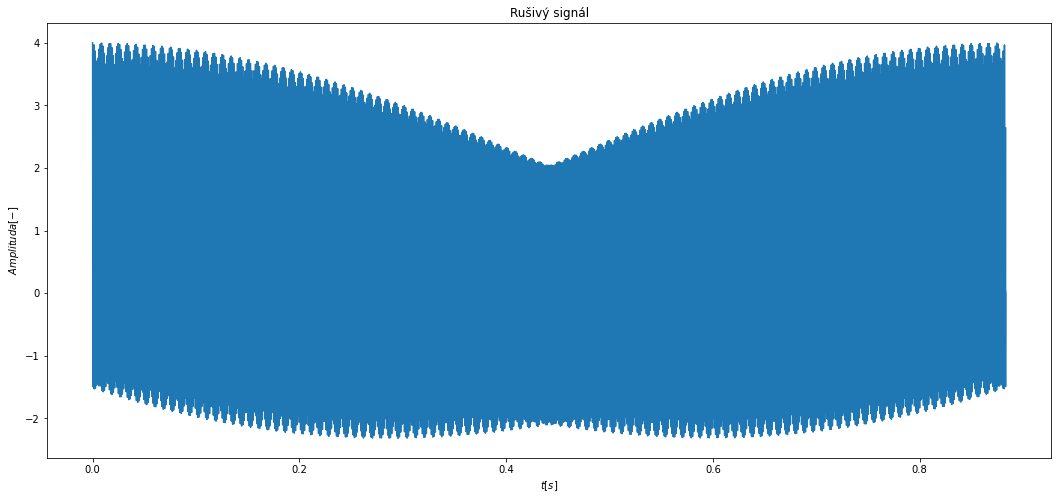
\includegraphics[scale=0.55,keepaspectratio]{Figure_25}
	\caption{Signál rušení}
\end{figure}
\end{landscape}

Můžeme vidět že signál nevypadá úplně přesně jako ve vstupním signálu a je to tím, že neznáme jeho amplitudu a počáteční fázy.
